Celem rozdziału jest przedstawienie testów aplikacji oraz sposobów jej obsługi. Zostały w nim umieszczone przykładowe sposoby korzystania z aplikacji. Przedstawiono również funkcjonowanie zaimplementowanych funkcji odpowiadających za uzyskanie odpowiedzi od maszyny.
\section{Obsługa aplikacji}
Do zaimplementowania całego działania aplikacji skorzystano z edytora kodu źródłowego Visual Studio Code. Za pomocą tego oprogramowania możliwe jest przeprowadzanie testów bądź debugowanie stworzonego projektu. Visual Studio Code jest edytorem dostępnym na wielu systemach operacyjnych takich jak Windows czy Linux. W celu przeprowadzenia testów poprawności działania aplikacji wykonano szereg operacji, które pozwoliły na ocenę działania zaimplementowanego kodu. Visual Studio Code umożliwia uruchomienie aplikacji webowej za pomocą przeglądarki internetowej. Możliwe było przeprowadzenie badań nad funkcjonalnością aplikacji. Poprzez stworzenie kilku użytkowników, przeprowadzone zostały testy nad komunikacją tekstową z maszyną i sprawdzenie czy uzyskana zostanie odpowiedź na przesłane komendy.
\section{Zaimplementowane polecenia}
Głównym założeniem projektu była komunikacja z maszyną poprzez wpisywanie odpowiednich komend w języku naturalnym. Miały one na celu uzyskanie odpowiedzi przez mikrokontroler w postaci odpowiednich czynności. Wiadomości wpisane w komunikatorze miały spowodować uruchomienie danego elementu wykonawczego podłączonego od określonego pinu GPIO. W celu przeprowadzenia takiej komunikacji dokonano translacji funkcji na odpowiednie komendy napisane w języku naturalnym, które powodowały uzyskanie takiego wyniku. W aplikacji zaimplementowano polecenia takie jak:
\begin{itemize}  
	\item \textbf{red on}, komenda ta powoduje włączenie się diody LED i zaświecenie kolorem czerwonym
	\\
	\item \textbf{green on}, komenda ta powoduje włączenie się diody LED i zaświecenie kolorem zielonym
	\\
\item \textbf{yellow on}, komenda ta powoduje włączenie się diody LED i zaświecenie kolorem żółtym
	\\
\item \textbf{stop red}, komenda ta powoduje wyłączenie diody LED o kolorze czerwonym poprzez zmienienie stanu z wartości 1 na 0
	\\
	\item \textbf{stop green}, komenda ta powoduje wyłączenie diody LED o kolorze zielonym poprzez zmienienie stanu z wartości 1 na 0
	\\
\item \textbf{stop yellow}, komenda ta powoduje wyłączenie diody LED o kolorze żółtym poprzez zmienienie stanu z wartości 1 na 0
	\\
	\item \textbf{blink red}, komenda ta powoduje efekt migania diody LED o kolorze czerwonym
	\\
\item \textbf{blink green}, komenda ta powoduje efekt migania diody LED o kolorze zielonym
	\\
	\item \textbf{blink yellow}, komenda ta powoduje efekt migania diody LED o kolorze żółtym
	\\
\item \textbf{flowing leds}, komenda ta powoduje uzyskanie efektu wizualnego ruchu diod
	\\
	\item \textbf{run servo}, komenda ta pozwala na sterowanie serwomechanizmem
	\\
\item \textbf{sequential}, komenda ta powoduje sekwencyjne wykonywanie się poleceń, które spowodują uruchomienie zainstalowanych elementów wykonawczych, jeden po drugim
	\\
	\item \textbf{turn on all},komenda powoduje włączenie wszystkich trzech diod LED.
	\\
\item \textbf{turn off all}, komenda powoduje wyłączenie wszystkich trzech diod LED
	\\
\end{itemize}
\newpage
\section{Zarządzanie komunikatorem}
W celu możliwości dołączenia do czatu, użytkownik musi wpisać swoją nazwę pod którą będzie widoczny oraz nazwę pokoju. Dane te muszą zostać wypełnione w odpowiednich polach tekstowych. Jeżeli użytkownik zostawi puste pole, w którym musi wpisać swoją nazwę lub nazwę pokoju, nie będzie on miał dostępu do zalogowania się do komunikatora.
\begin{figure}[htbp]
	\centering
	\includegraphics[width=0.5\linewidth]{"obrazy/TESTLOGOWANIE"}
	\caption{Formularz logowania użytkownika do aplikacji}
	\label{fig:39}
\end{figure}
\begin{figure}[htbp]
	\centering
	\includegraphics[width=0.5\linewidth]{"obrazy/TESTnazwapokoju"}
	\caption{Próba dołączenia do komunikatora}
	\label{fig:40}
\end{figure}
\newpage
W celach testowych wpisano jedynie nazwę pokoju do którego użytkownik chciałby dołączyć. Pole tekstowe zawierające nazwę użytkownika, pod którą chciałby być wyświetlany zostało pominięte. Przy braku wypełnienia wszystkich danych, nie został uzyskany dostęp do zalogowania się do komunikatora poprzez pojawienie się przycisku, który przekierowałby użytkownika do czatu.
W momencie kiedy użytkownik wypełni wszystkie potrzebne dane, w aplikacji pojawi się przycisk umożliwiający zalogowanie się do aplikacji. Poprzez kliknięcie przycisku Zaloguj, użytkownik zostanie przekierowany do komunikatora tekstowego.

\begin{figure}[htbp]
	\centering
	\includegraphics[width=0.5\linewidth]{"obrazy/TESTdolaczenie"}
	\caption{Logowanie do komunikatora}
	\label{fig:41}
\end{figure}
Po wypełnieniu wymaganych danych i kliknięciu przycisku logowania, użytkownik zostanie przekierowany do czatu. Tutaj będzie mógł nawiązać komunikację z maszyną poprzez wpisanie odpowiedniego tekstu.
W celu przeprowadzenia dodatkowych testów stworzono drugiego użytkownika. Dołączył on do pokoju czatu z tą samą nazwą co poprzedni użytkownik. Wykonanie takiej operacji pozwoli na możliwość korzystania z komunikatora przez kilku zalogowanych klientów.
\newpage
\begin{figure}[htbp]
	\centering
	\includegraphics[width=0.5\linewidth]{"obrazy/TEST2uzytkownik"}
	\caption{Tworzenie drugiego użytkownika}
	\label{fig:43}
\end{figure}
\begin{figure}[htbp]
	\centering
	\includegraphics[width=0.5\linewidth]{"obrazy/TESTczatpodolaczeniu"}
	\caption{Interfejs użytkownika po zalogowaniu}
	\label{fig:42}
\end{figure}
Na Rysunku \ref{fig:44} została przedstawiona perspektywa użytkownika o nazwie user1. Wiadomości wysłane przez klienta user2 wyświetlane są po lewej stronie interfejsu wyróżnione szarym tłem. Drugi użytkownik wpisując polecenie flowing leds przesłał żądanie do mikrokontrolera co wynikiem było uzyskanie efektu płynącej diody. Wiadomość ta została zapisana w archiwum i użytkownik pod nazwą user1, który zalogował się do tego samego pokoju może zobaczyć wysłane wiadomości. 
\newpage.
\begin{figure}[htbp]
	\centering
	\includegraphics[width=0.5\linewidth]{"obrazy/TESTpisaniewiadomosci"}
	\caption{Testowanie komunikacji tekstowej}
	\label{fig:44}
\end{figure}

Na Rysunku \ref{fig:46} zostały przedstawione obie perspektywy. Ukazują one jak widoczne są wiadomości wpisane przez określonego użytkownika. Oba te polecenia wysłane przez klientów zostały zapisane w archiwum i po ponownym zalogowaniu się do czatu o tej samej nazwie pokoju, klienci czatu będą w stanie odtworzyć wiadomości, które zostały przez nich wysłane. Użytkownik o nazwie user1 wpisał polecenie o nazwie run servo i wiadomość ta pojawiła się w czacie po obu stronach. Komenda ta umożliwia sterowanie serwomechanizmem, który przesuwa się o określony kąt do momentu osiągnięcia zadanej pozycji.

\begin{figure}[htbp]
	\centering
	\includegraphics[width=0.5\linewidth]{"obrazy/TESTwidok2interfejsysequential"}
	\caption{Sekwencyjnie wykonywanie się zaimplementowanych metod}
	\label{fig:46}
\end{figure}
\newpage
Użytkownik o nazwie user2 wpisał polecenie o treści sequential. Powoduje to sekwencyjne wykonywanie się zaimplementowanych metod, które odpowiedzialne są za uruchomienie zainstalowanych elementów elektronicznych przy komunikacji z mikrokontrolerem. Wiadomość ta jest widoczna w obu perspektywach. 

\begin{figure}[htbp]
	\centering
	\includegraphics[width=0.5\linewidth]{"obrazy/TESTuser3"}
	\caption{Widok komunikatu o opuszczeniu czatu przez użytkownika}
	\label{fig:47}
\end{figure}

Dodatkowo zaimplementowano mechanizm, który będzie sygnalizował opuszczenie użytkownika z czatu. W tym celu stworzono kolejnego klienta, który dołączył do czatu, a następnie go opuścił. Komunikat został wysłany do użytkowników, którzy korzystają wciąż z komunikatora. Zostali oni poinformowani o tej sytuacji.
\begin{figure}[htbp]
	\centering
	\includegraphics[width=0.5\linewidth]{"obrazy/TESTflowingleds"}
	\caption{Interfejs zawierający archiwum wiadomości}
	\label{fig:48}
\end{figure}

Po wpisaniu większej liczby wiadomości, okno komunikatora zacznie się przewijać ukazując najwcześniejsze wysłane polecenia. Zaimplementowano mechanizm, który pozwoli na przewijanie wiadomości interfejsu czatu.
\newpage
Kliknięcie przycisku zamykającego komunikator znajdujący się po prawej stronie paska nawigacyjnego przekieruje nas ponownie do formularza.  Będziemy musieli wypełnić ponownie pola tekstowego wymagające podanie nazwę użytkownika i pokoju by móc dołączyć do czatu. Po wpisaniu ponownie danych i zalogowaniu się jako użytkownik o nazwie user1 jesteśmy ponownie przekierowani do komunikatora w raz z całym archiwum wysłanych dotychczas wiadomości.
\begin{figure}[h]
\begin{subfigure}{0.5\textwidth}
\includegraphics[width=0.9\linewidth, height=6cm]{"obrazy/TESTLOGOWANIE"} 
\caption{Caption1}
\label{fig:subim1}
\end{subfigure}
\begin{subfigure}{0.5\textwidth}
\includegraphics[width=0.9\linewidth, height=6cm]{"obrazy/TESTostatniscreen"}
\caption{Caption 2}
\label{fig:subim2}
\end{subfigure}

\caption{Caption for this figure with two images}
\label{fig:image2}
\end{figure}



\newpage
\section{Przedstawienie uzyskanych wyników}
Poprzez wpisanie określonych komend w komunikatorze, użytkownik dostawał odpowiedzi od urządzenia w postaci działania poszczególnych elementów wykonawczych. Poniżej przedstawiono uzyskane wyniki przy wpisaniu polecenia:
\begin{itemize}  
	\item \textbf{turn on all}
	\begin{figure}[htbp]
	\centering
	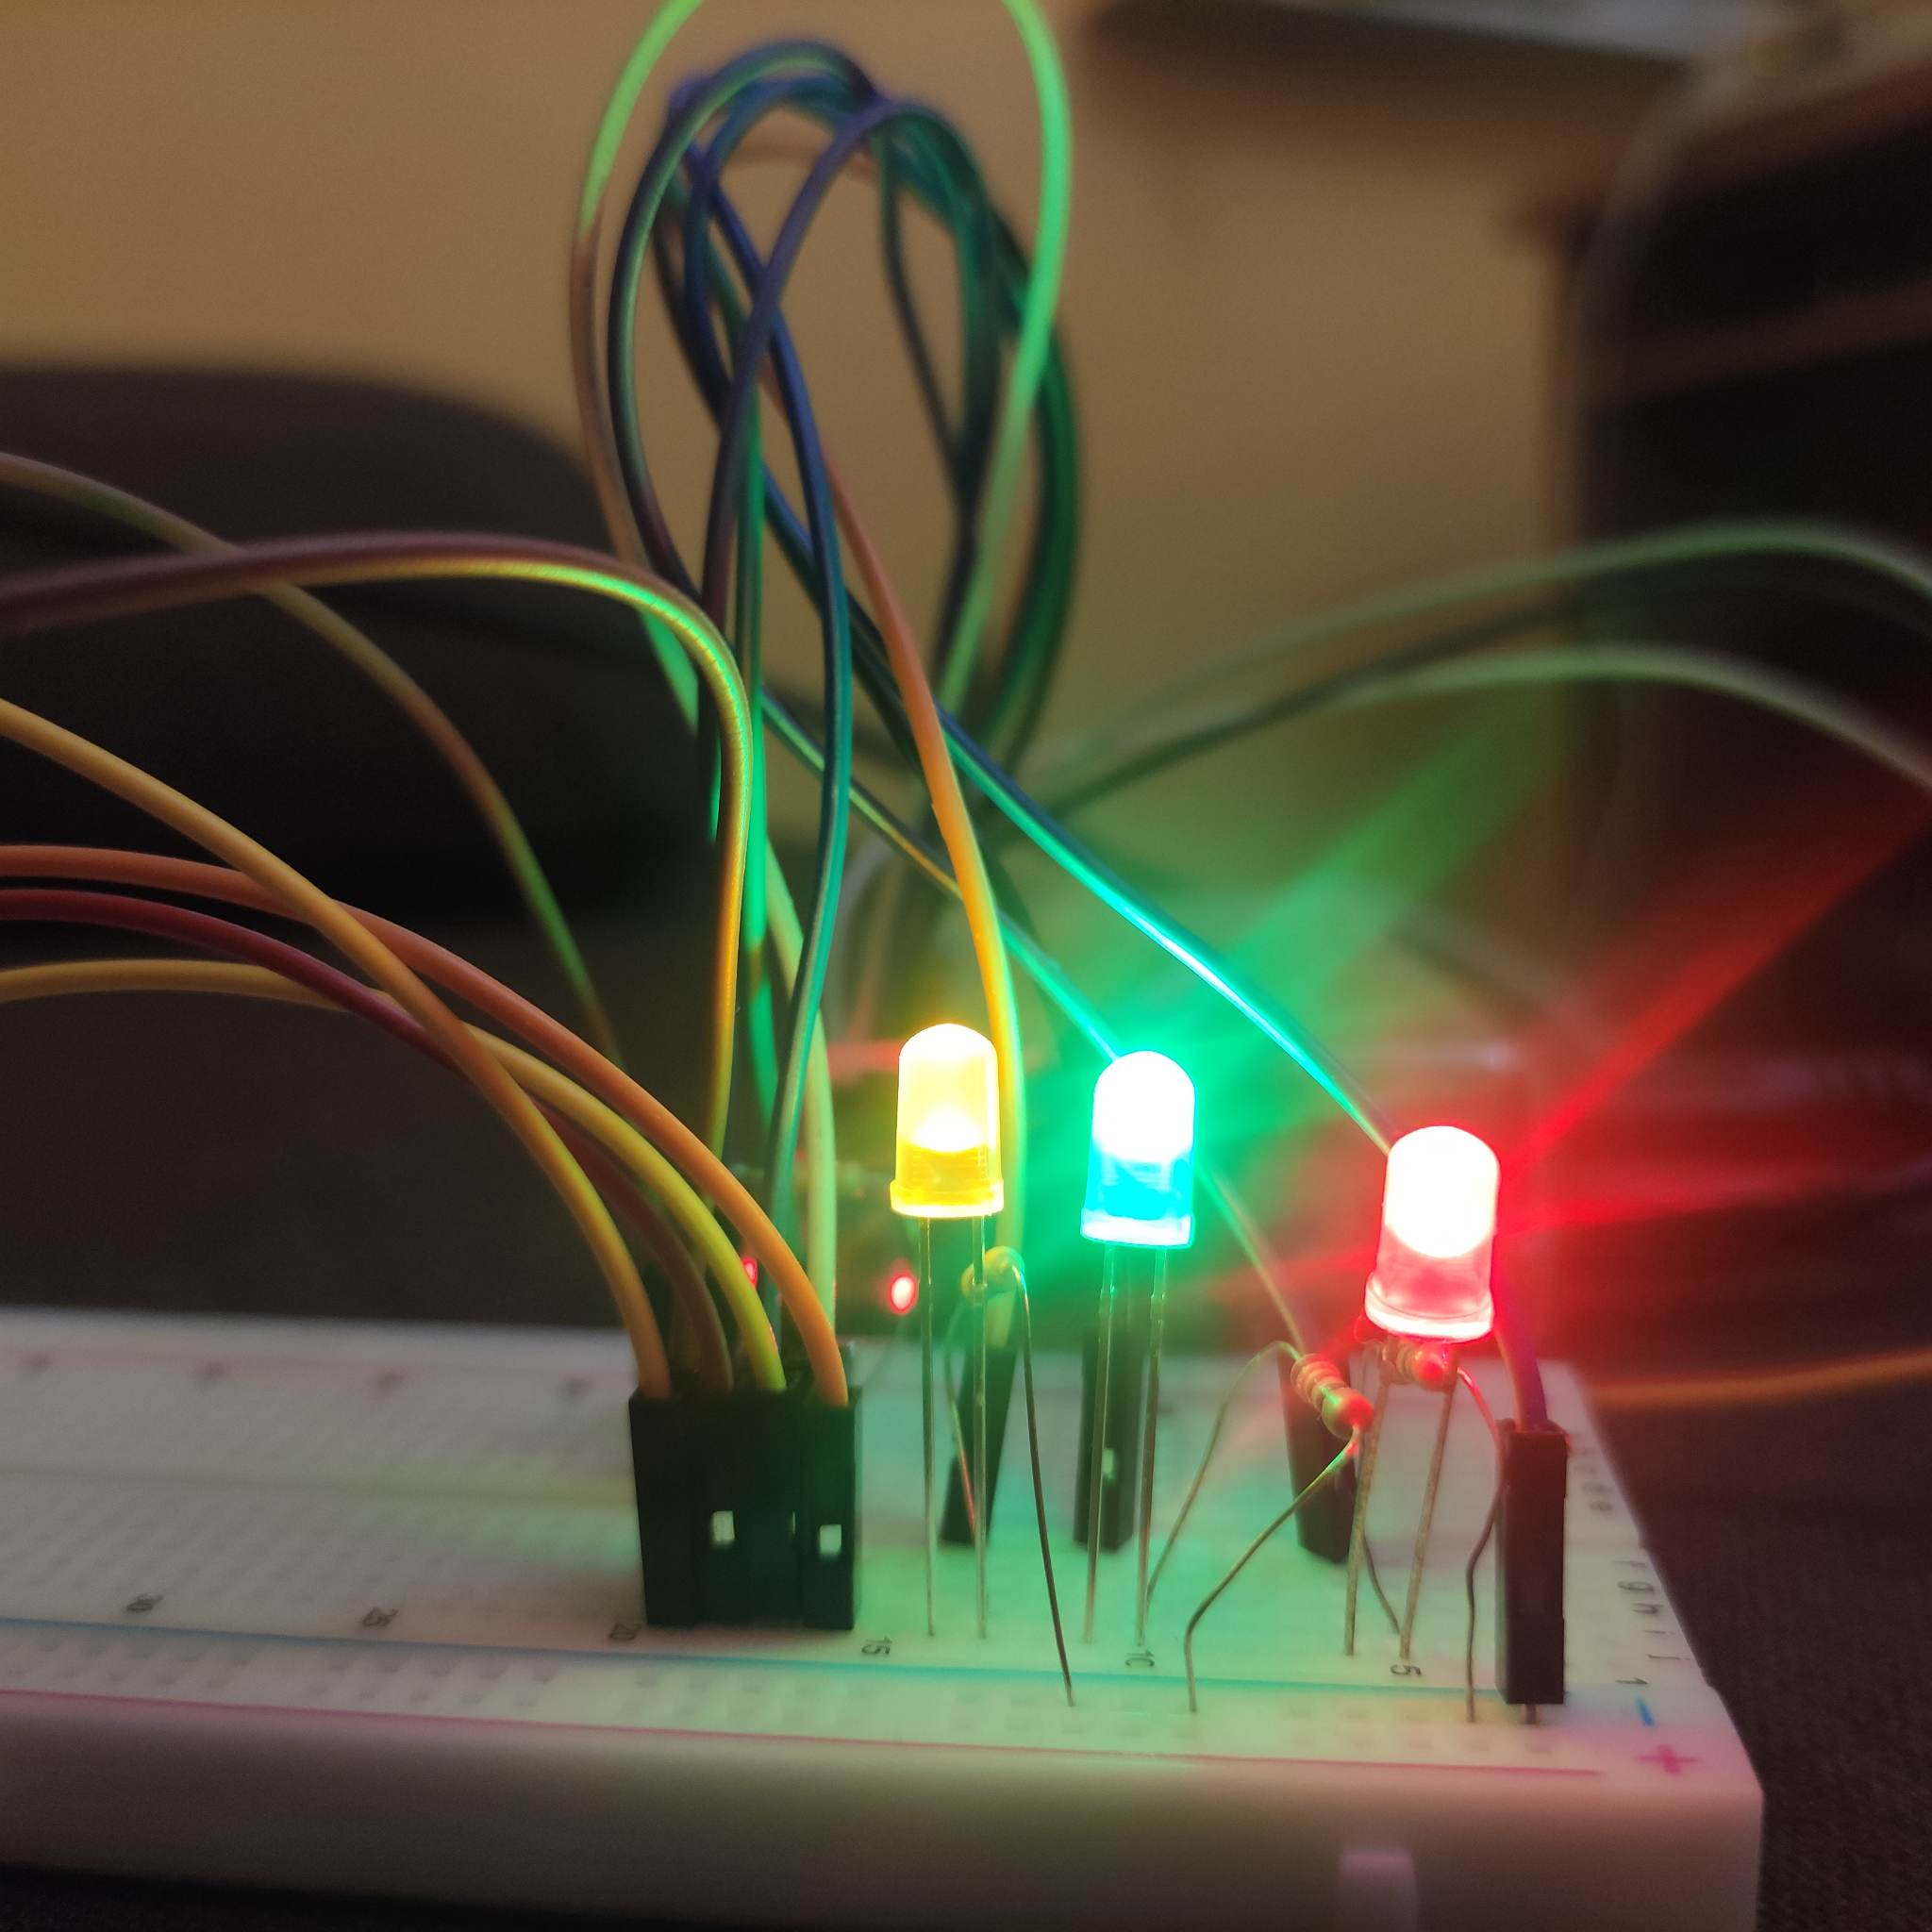
\includegraphics[width=0.4\linewidth, height=6cm]{"obrazy/turnonall.jpg"}
	\caption{Wywołanie komendy powodująca włączenie wszystkich diod}
	\label{fig:51}
\end{figure}
	\\
	\item \textbf{stop green}
	\begin{figure}[htbp]
	\centering
	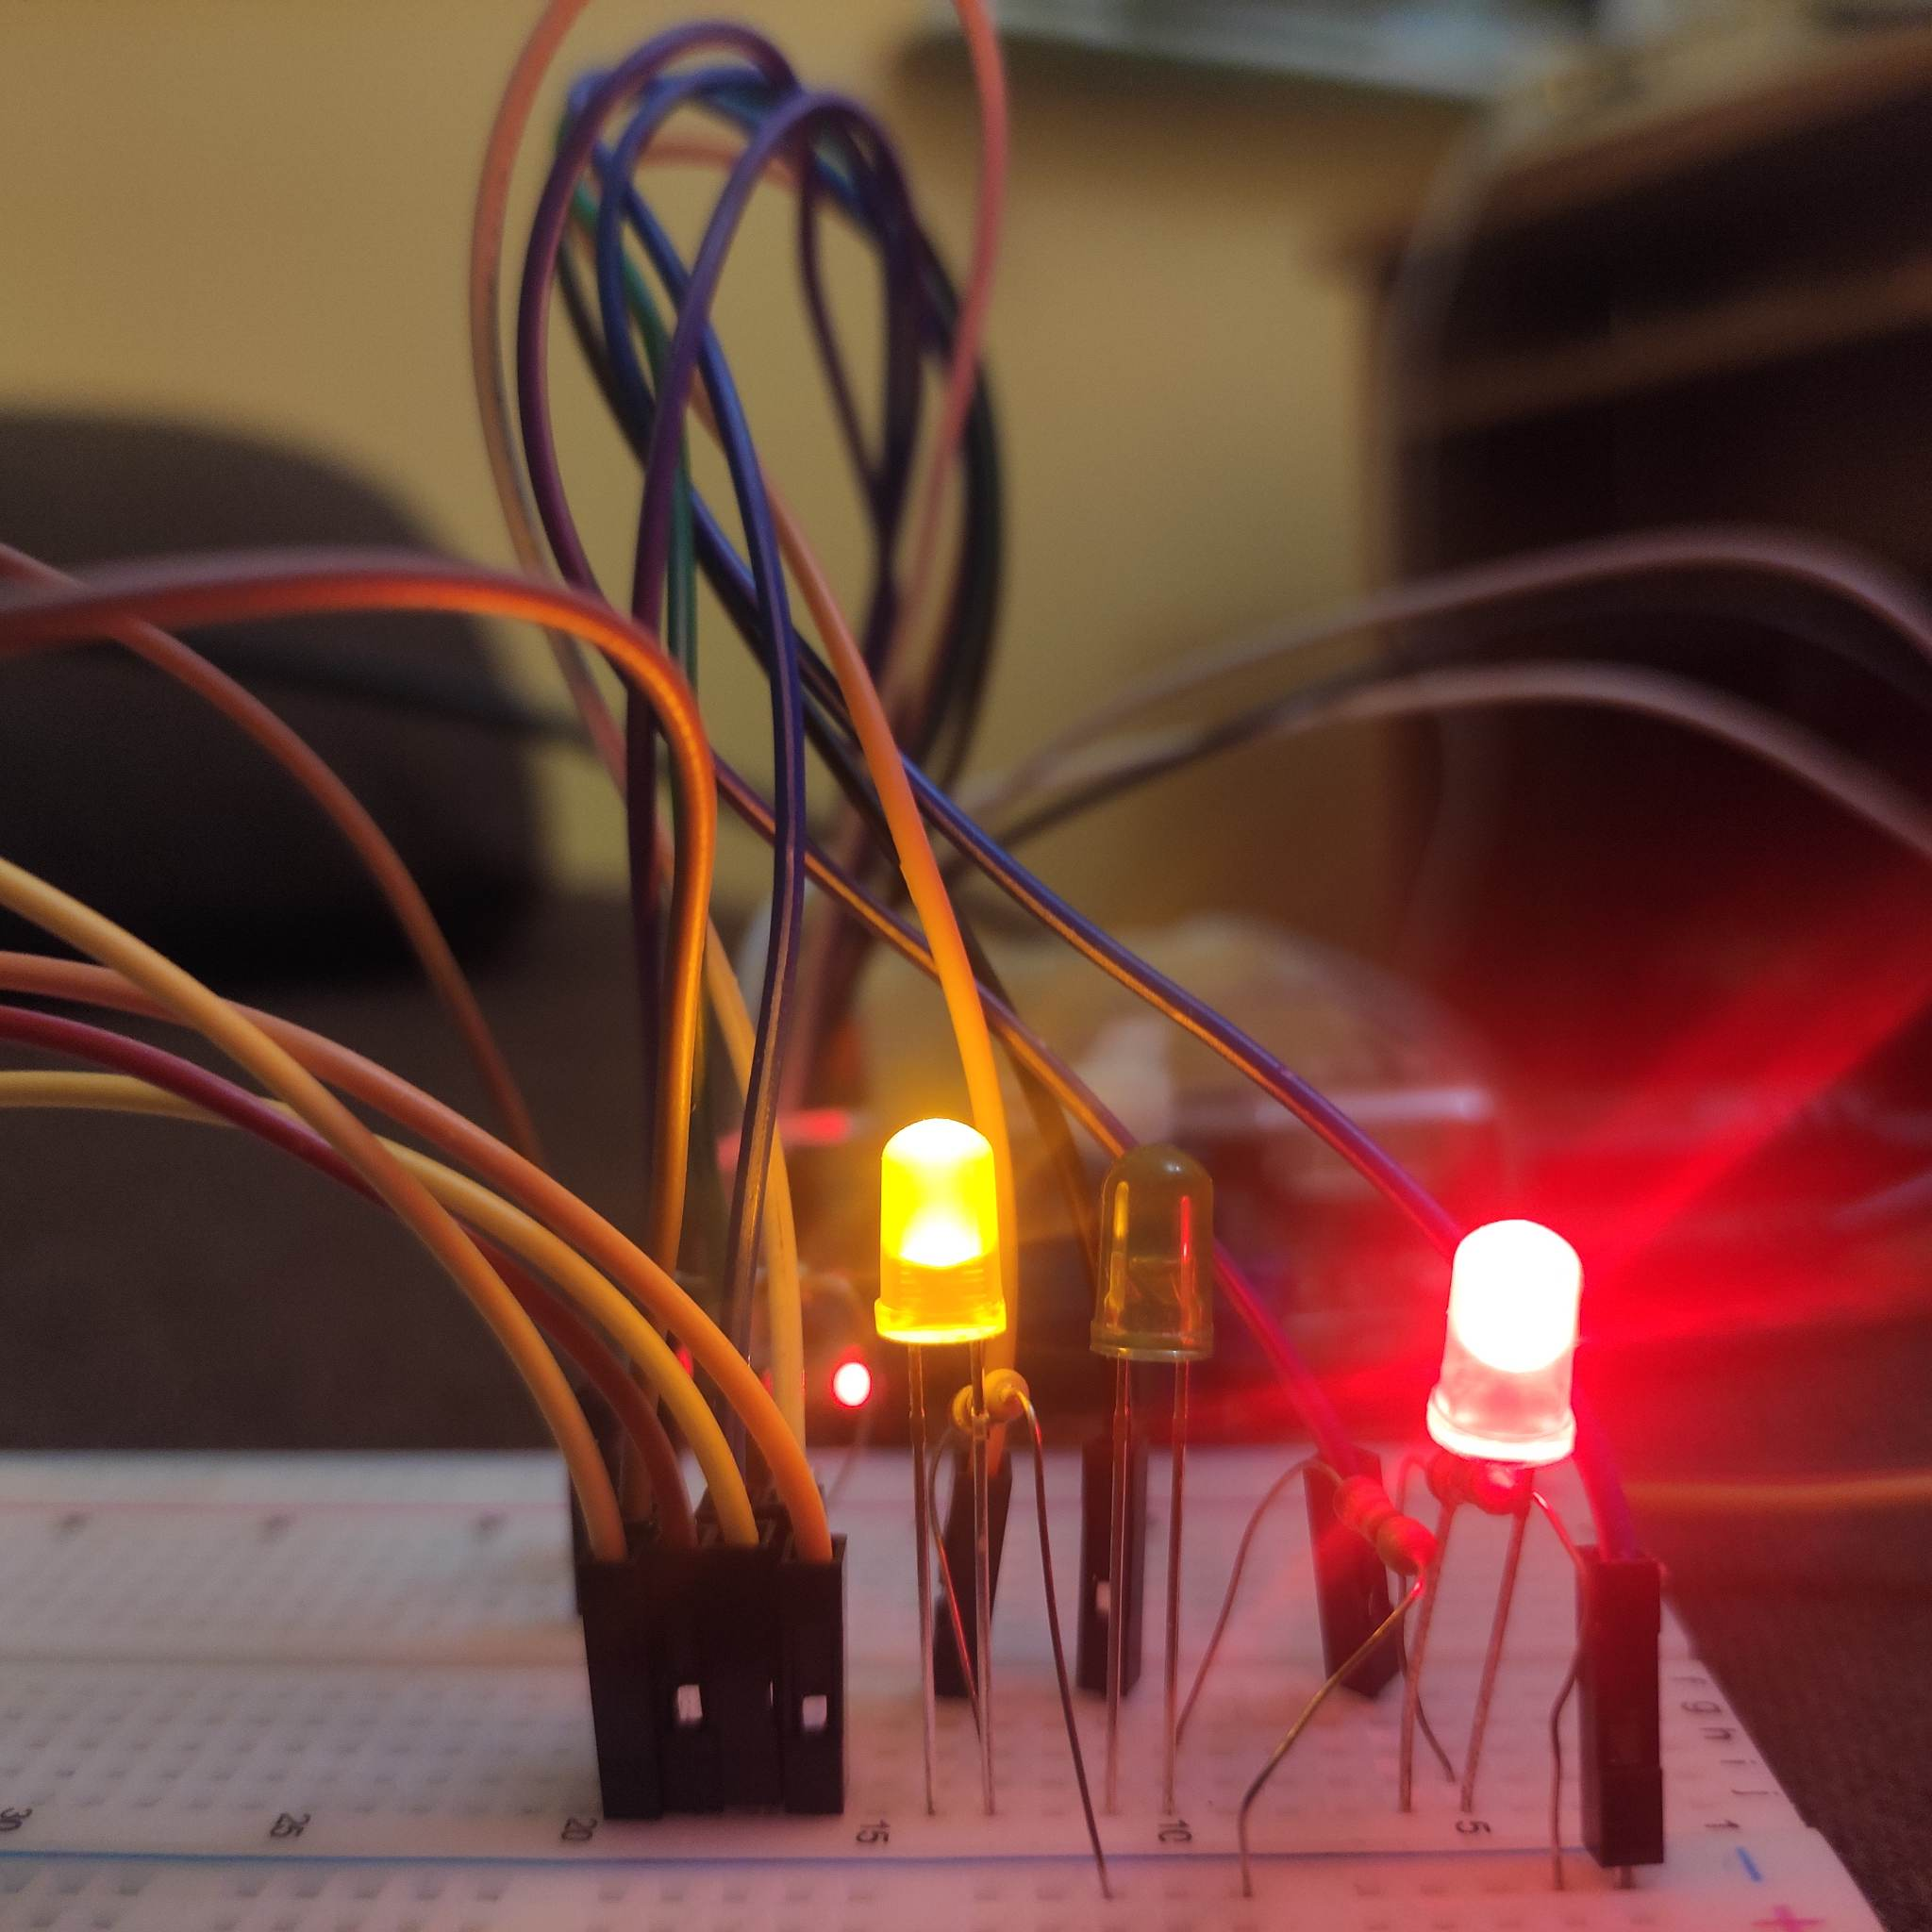
\includegraphics[width=0.4\linewidth, height=6cm]{"obrazy/stopgreen.jpg"}
	\caption{Wywołanie komendy powodująca wyłączenie diody o kolorze zielonym}
	\label{fig:52}
	\end{figure}
	\\
\newpage
\item \textbf{yellow on}
	\begin{figure}[htbp]
		\centering
		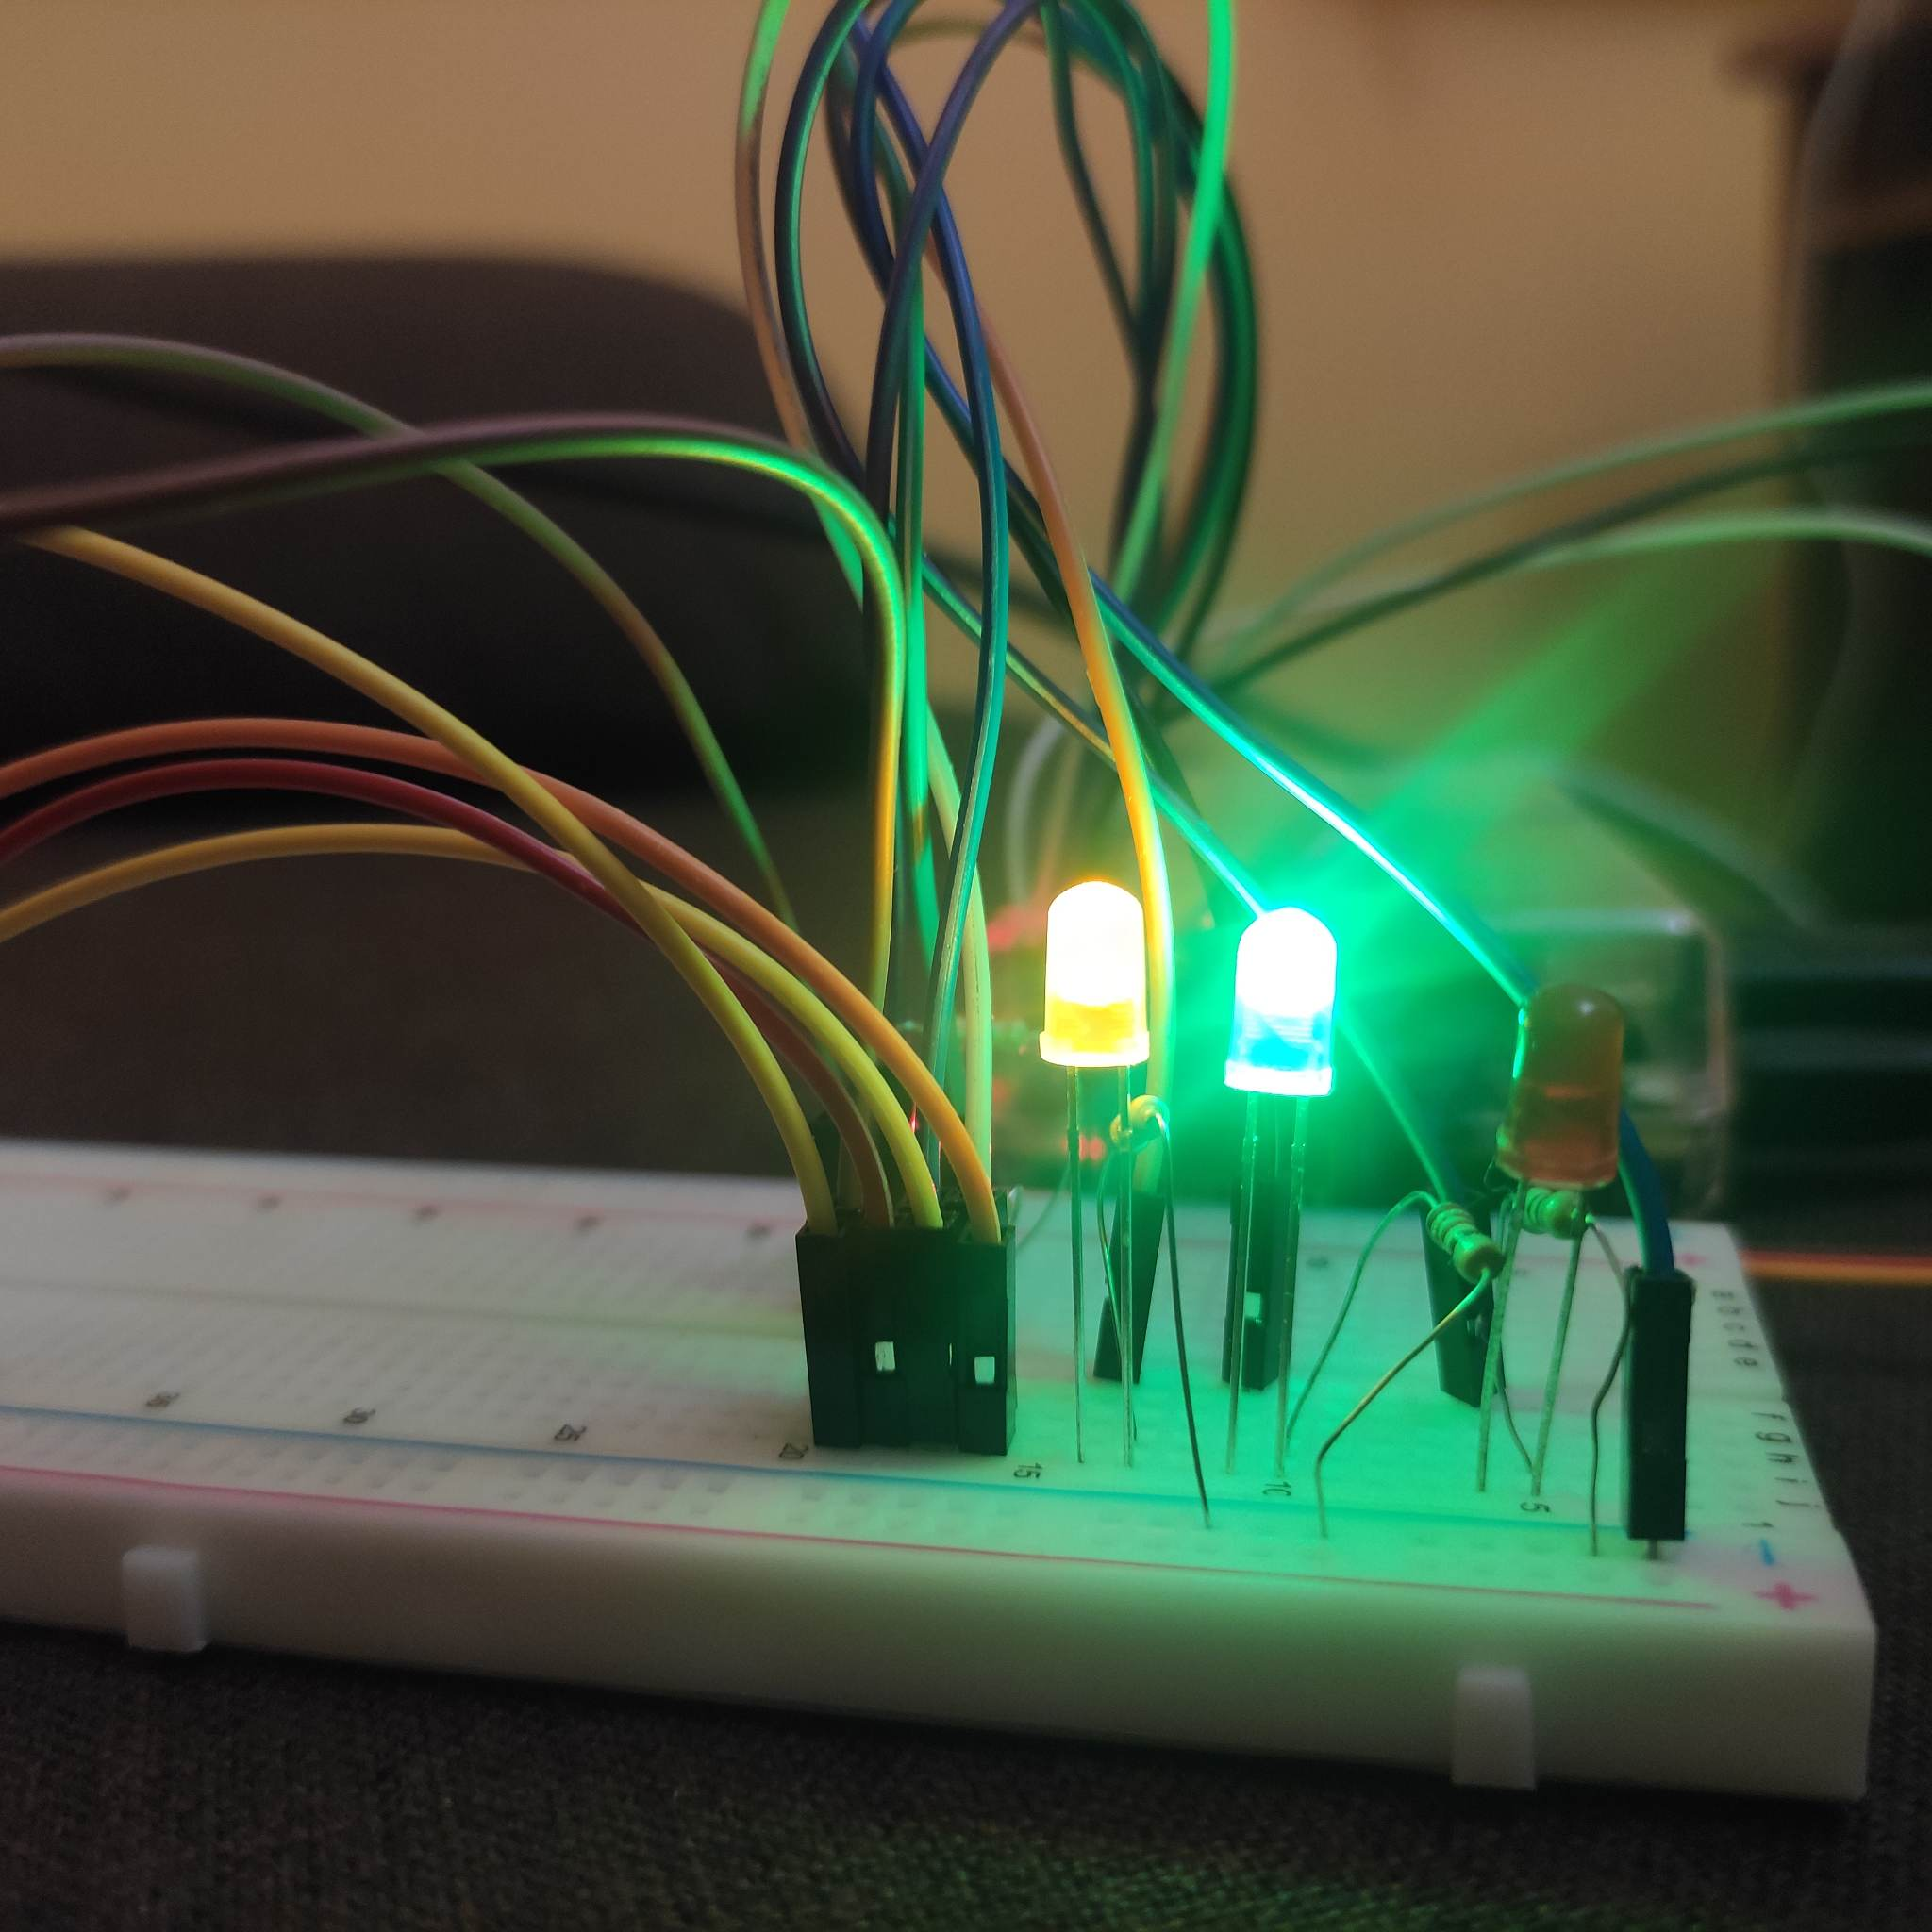
\includegraphics[width=0.4\linewidth, height=6cm]{"obrazy/yellowgreen.jpg"}
		\caption{Wywołanie komend  powodujących włączenie diod o kolorze żółtym i zielonym}
		\label{fig:54}
	\end{figure}
	\\
\item \textbf{turn off all}
	\begin{figure}[htbp]
	\centering
	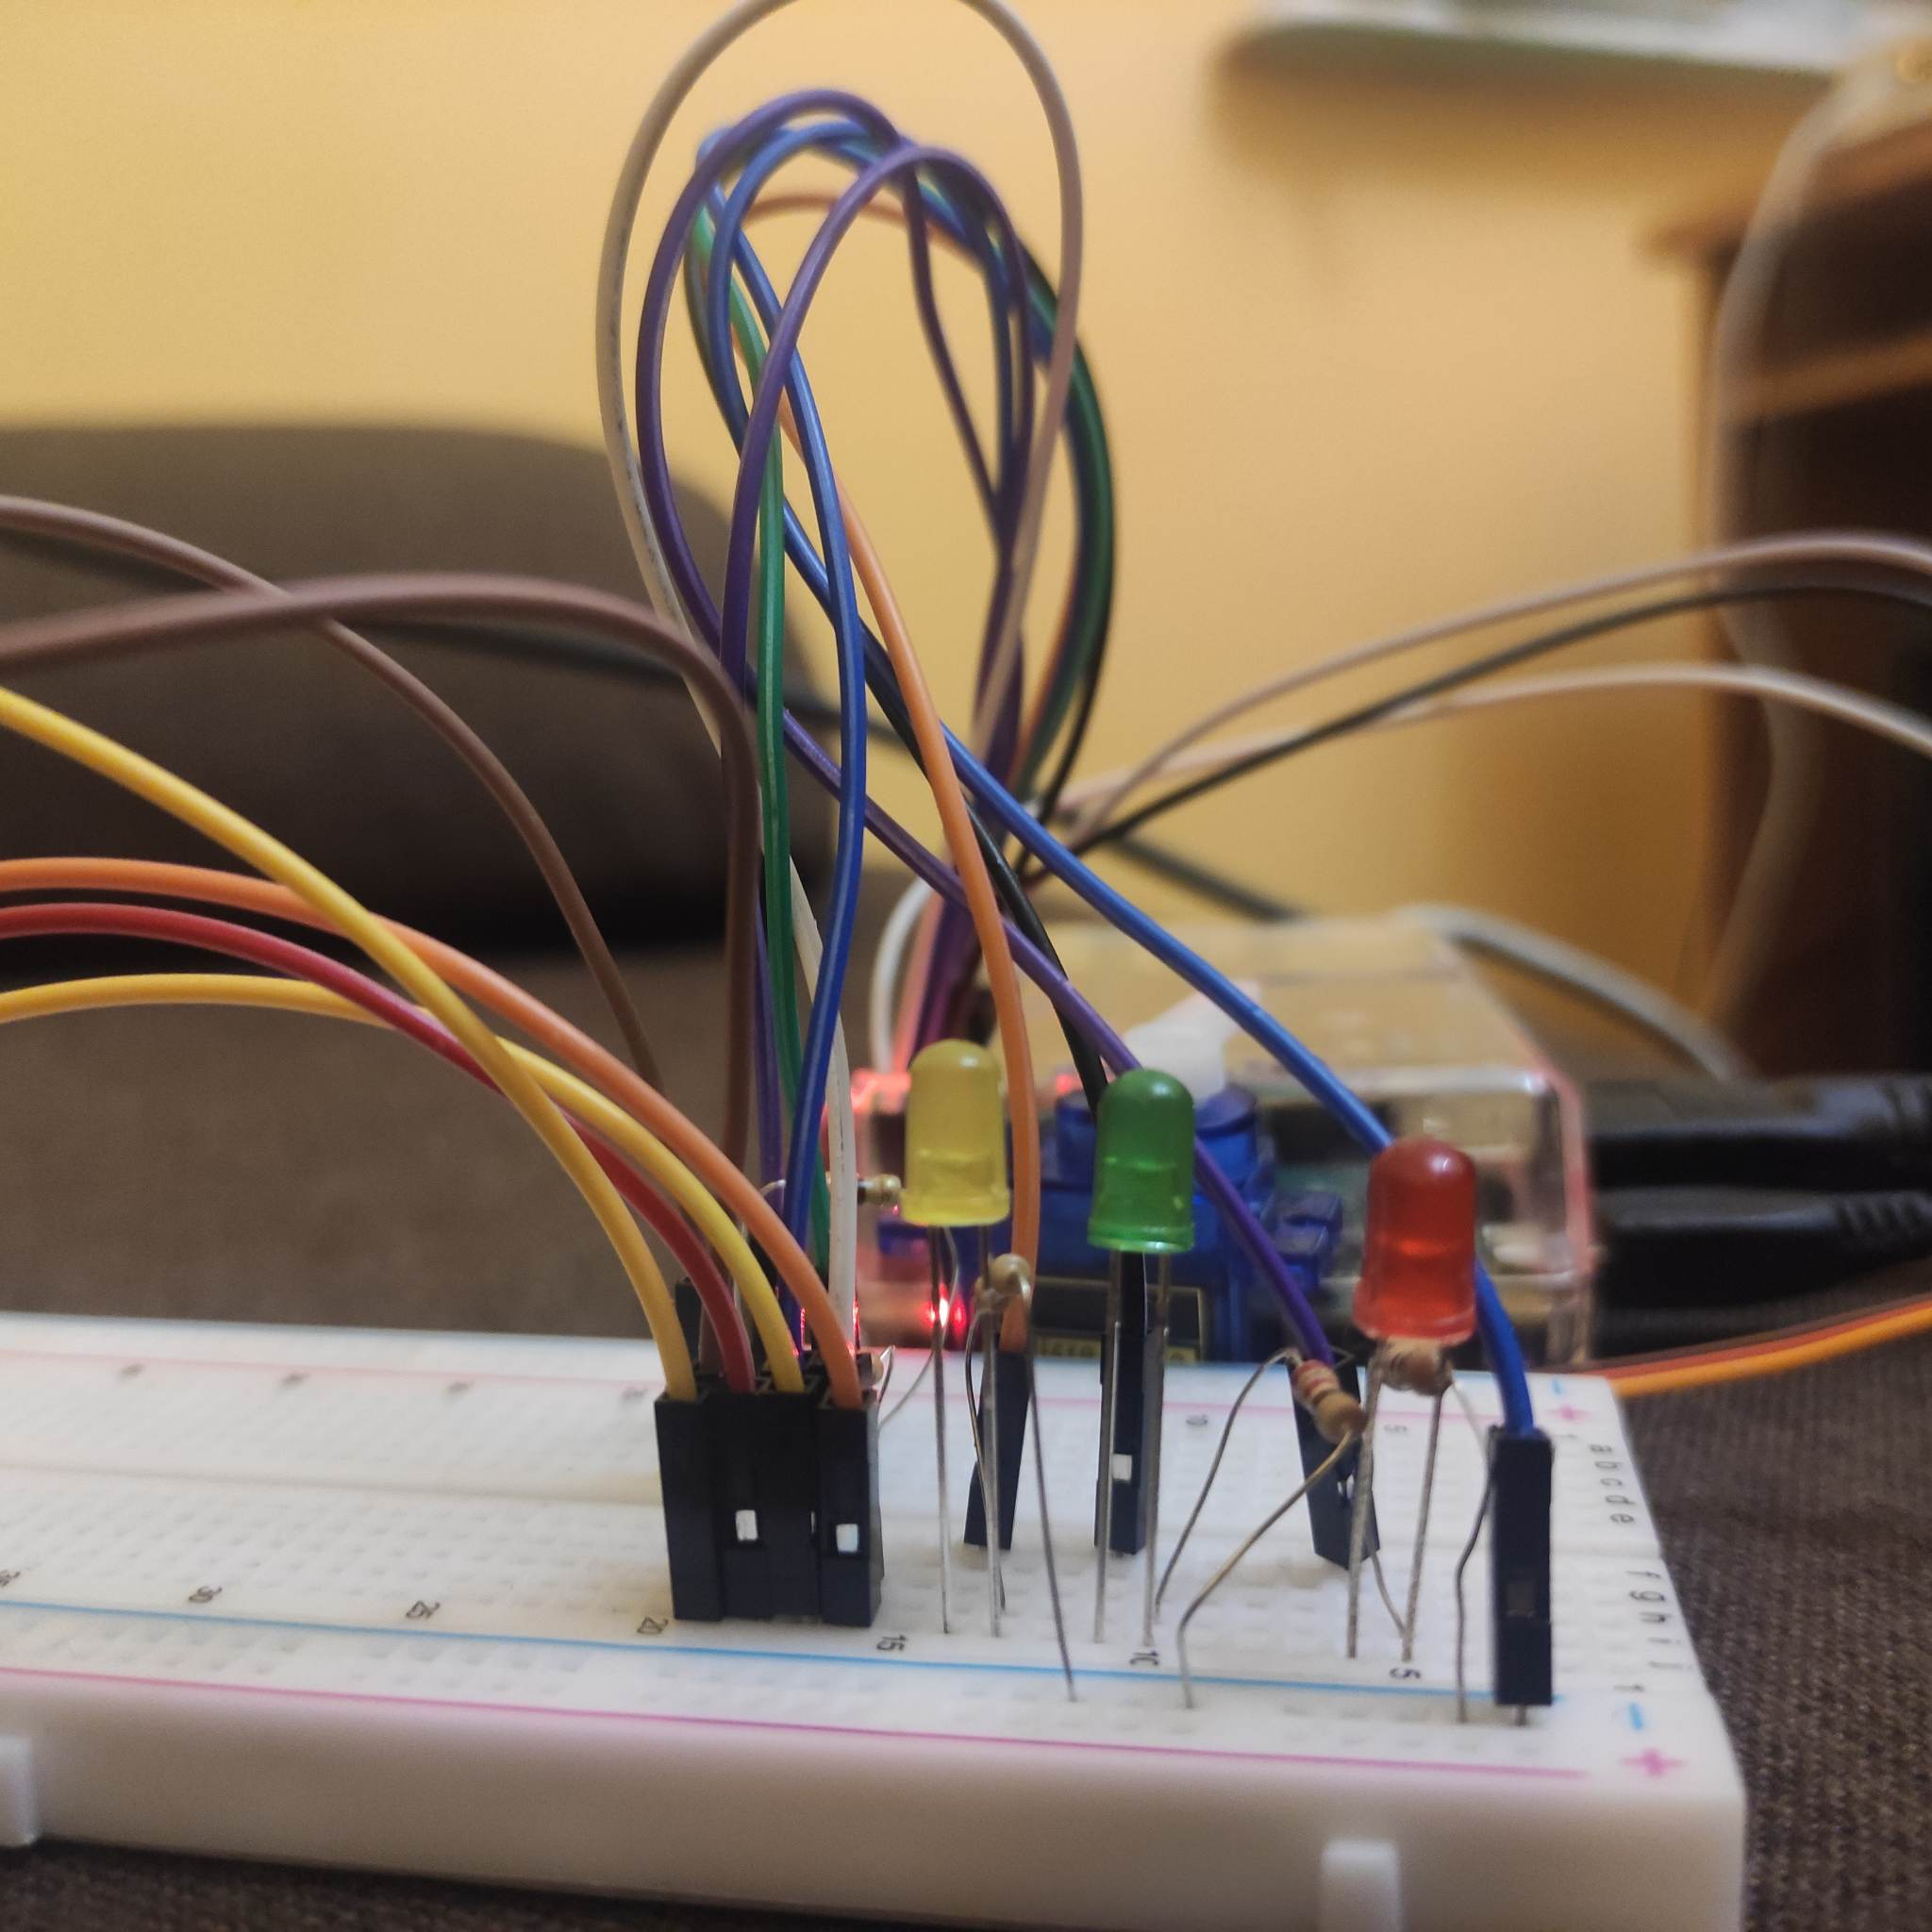
\includegraphics[width=0.4\linewidth, height=6cm]{"obrazy/turnoffall.jpg"}
	\caption{Wywołanie komendy powodująca wyłączenie wszystkich diod}
	\label{fig:53}
\end{figure}
	\\
\newpage
\item \textbf{run servo}
	\begin{figure}[htbp]
	\centering
	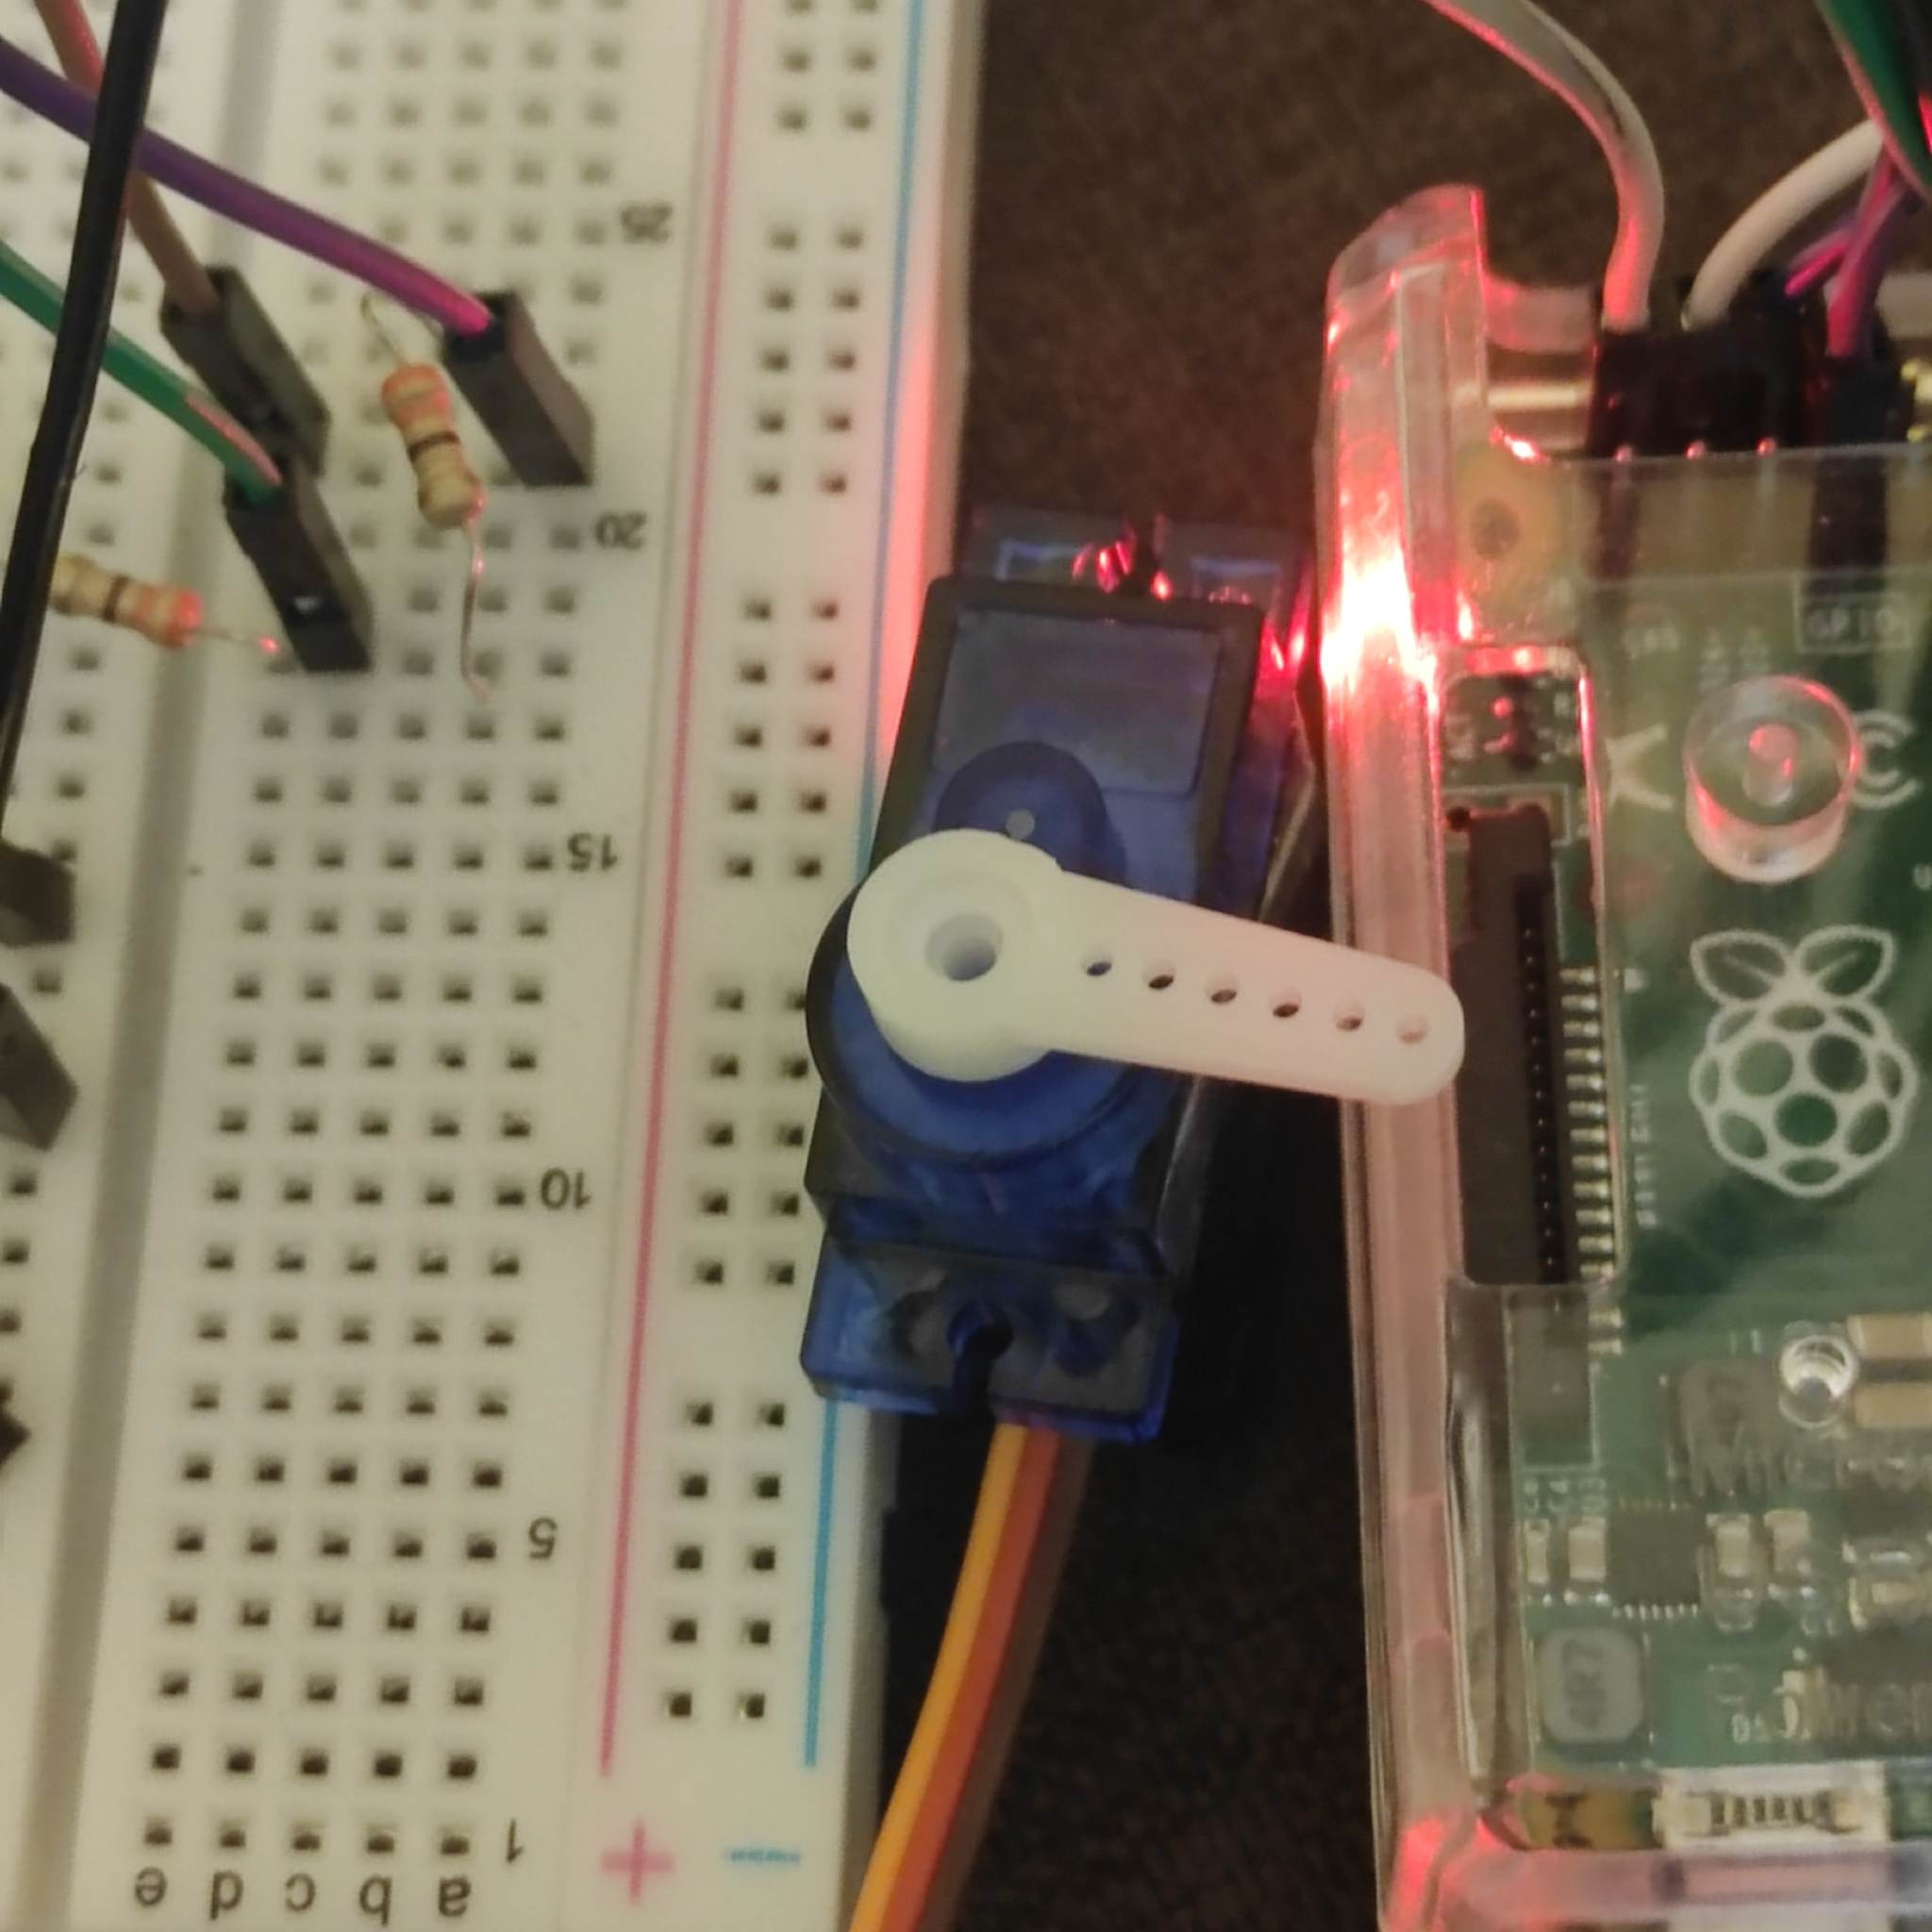
\includegraphics[width=0.4\linewidth, height=6cm]{"obrazy/servo1.jpg"}
	\caption{Pozycja początkowa serwomechanizmu}
	\label{fig:55}
\end{figure}
\begin{figure}[htbp]
	\centering
	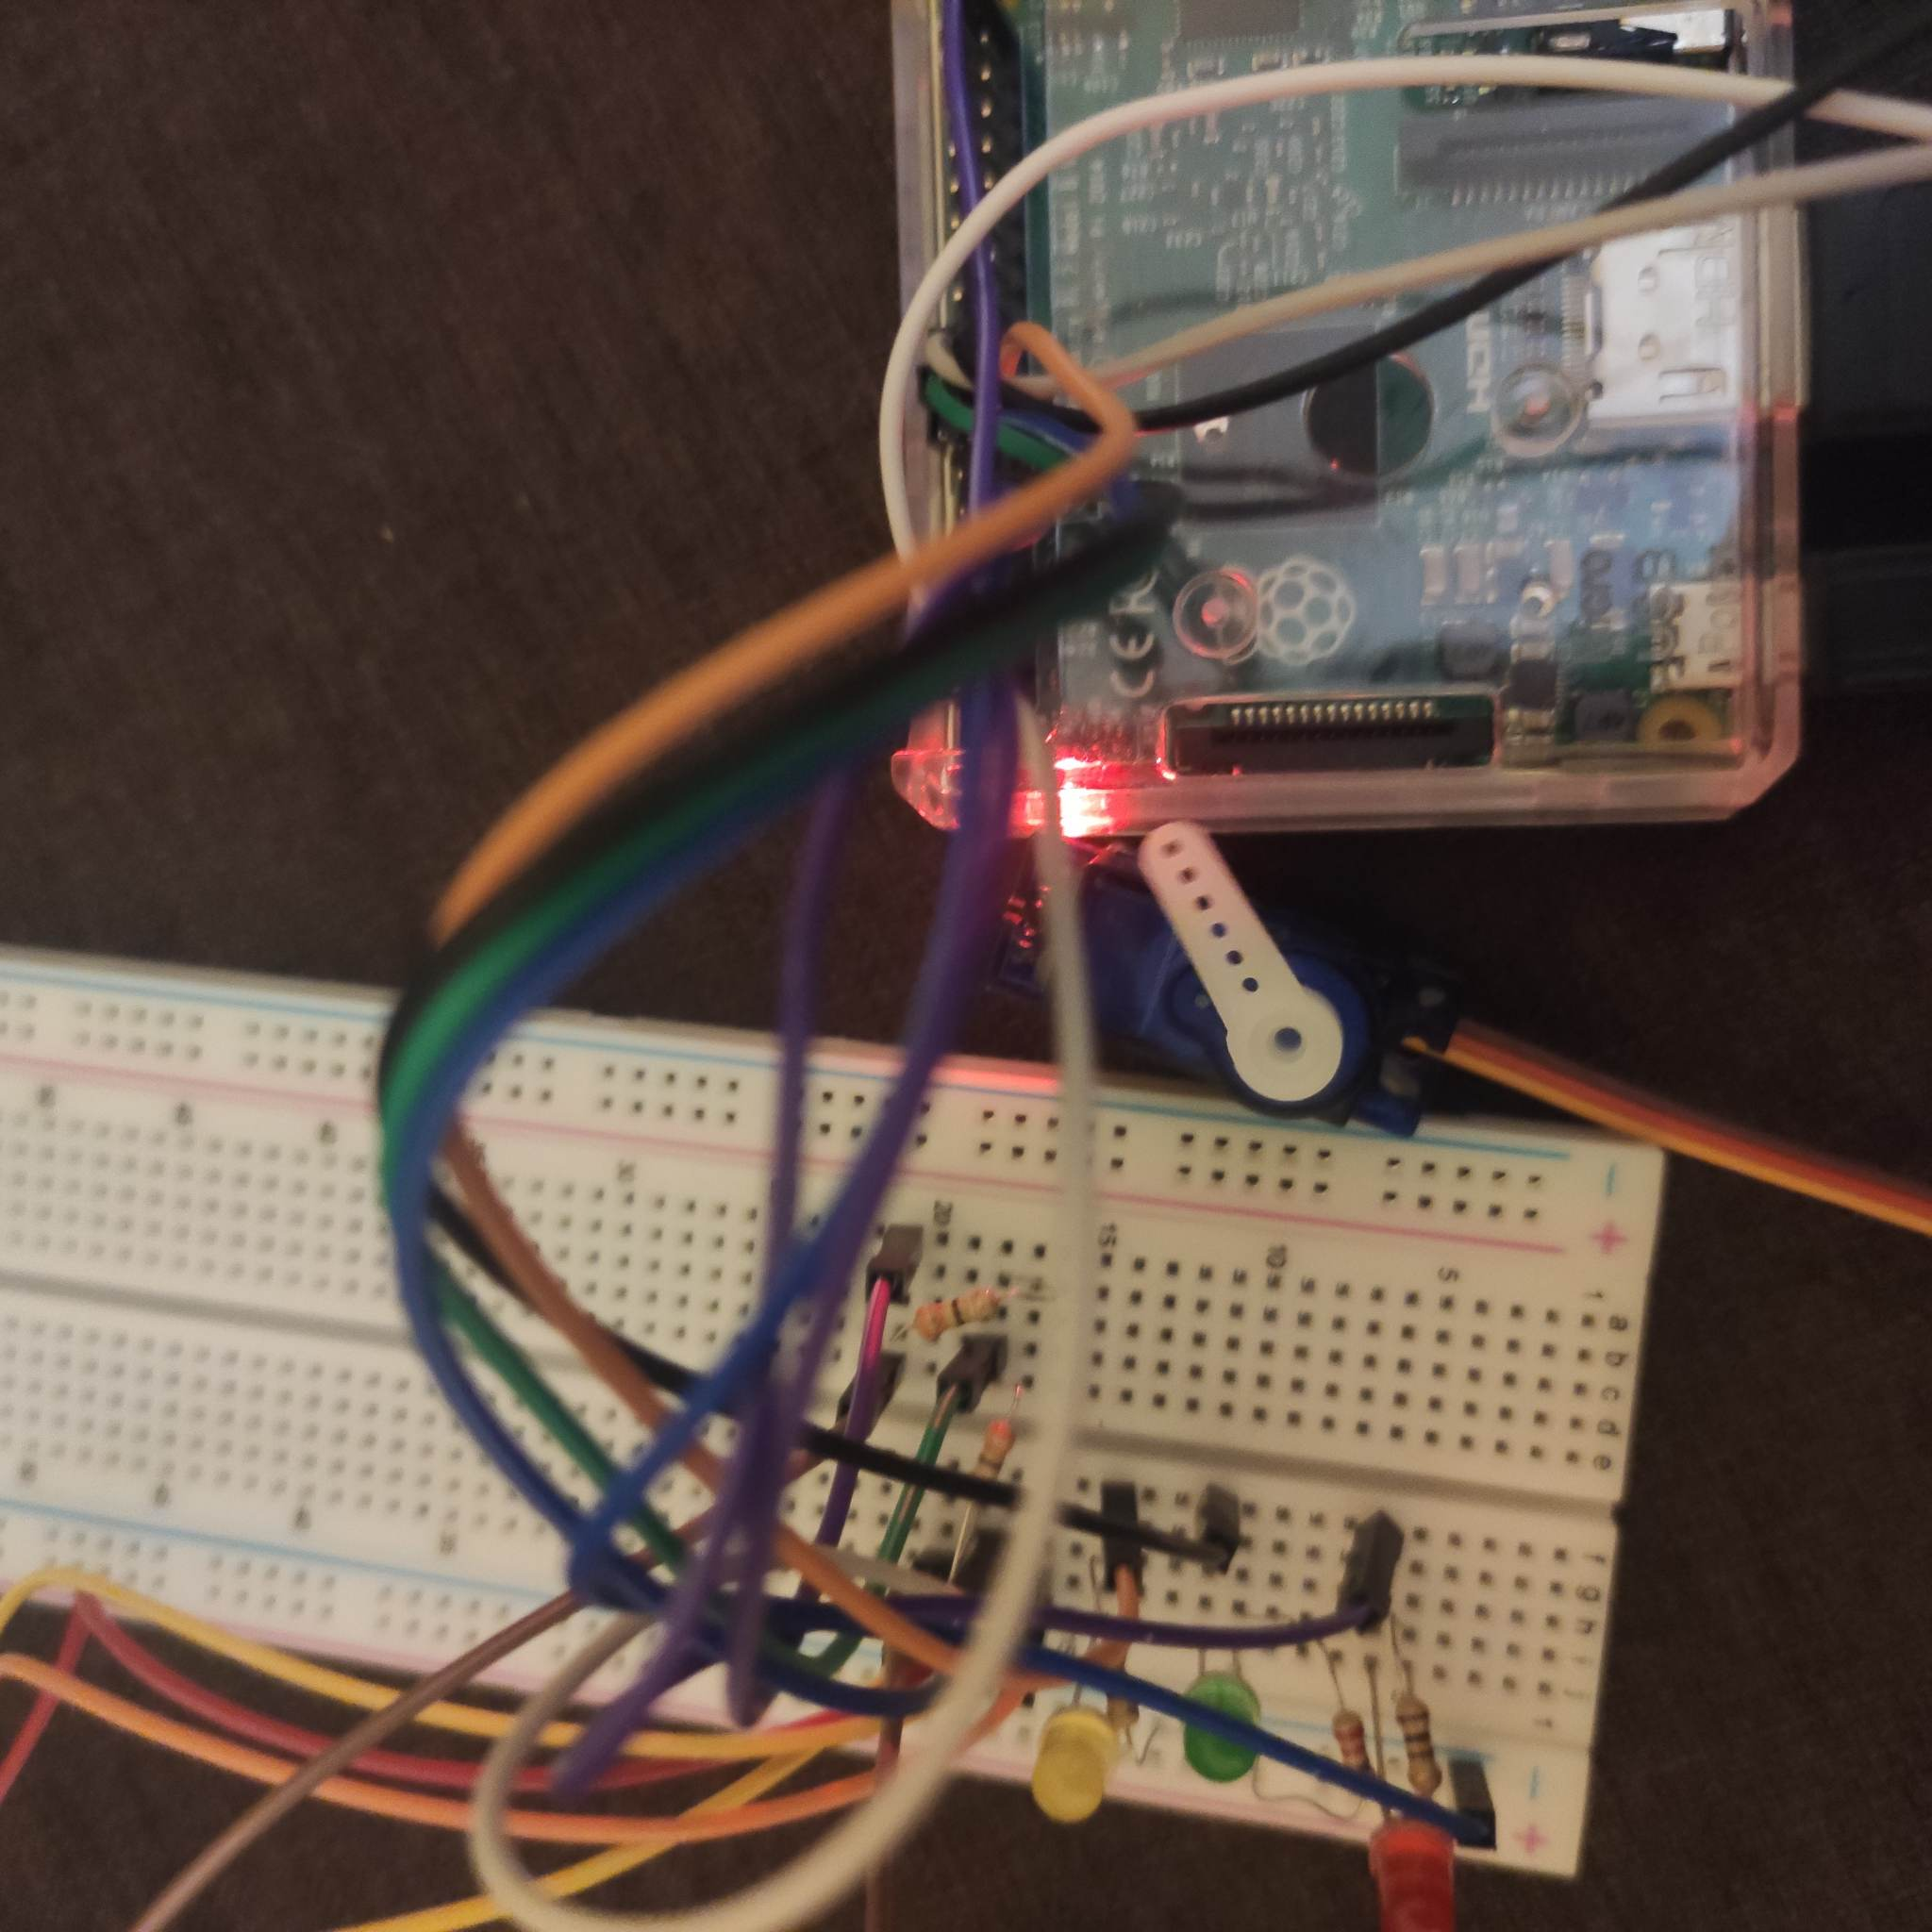
\includegraphics[width=0.4\linewidth, height=6cm]{"obrazy/servo2.jpg"}
	\caption{Wywołanie komendy umożliwiająca sterowanie serwomechanizmem }
	\label{fig:56}
\end{figure}
\\
\end{itemize}









